\begin{figure}[ht]
  \caption{The WolfTutor starting screen} 
  \centering
    \label{fig:start_screen}
    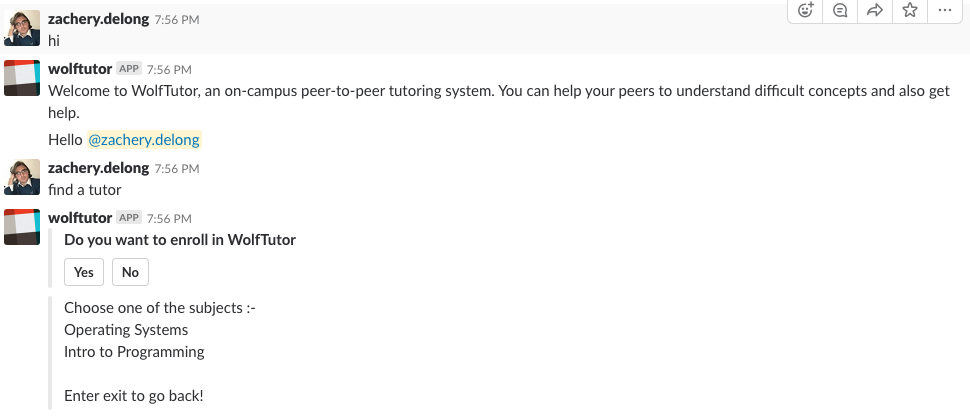
\includegraphics[width=0.5\textwidth]{fig_start_screen.png}
\end{figure}

WolfTutor is a system that seeks to enable students to tutor other students in a
course-setting. It is a slack-based chat app that attempts to connect potential
tutors in given subjects with students who need help with those subjects. Put
another way, WolfTutor is an applicatio nthat focuses entirely on enabling 
peer tutoring. At first blush, it seems like the app is an app to actually
facilitate peer tutoring, which is not entirely accurate. WolfTutor has
functions to register tutors and students and to schedule tutoring sessions. It
does not have functionality to actually perform the tutoring itself, but is a
logistic tool to enable the coordination required to schedule tutoring sessions.

WolfTutor is also gamified. It rewards tutors who are highly rated with a points
system which can be implemented in a number of different contexts to help
incentivize students to tutor other students.

There are a number of things that WolfTutor does extremely well, chief among
them its novel interface.  Being a chatbot makes the application easy to port to
new languages and new devices, since its entire UI consists of simple english
sentences and some rudimentary web inputs like text boxes and drop-downs.  That
being said, there are a few potential areas for improvement, chief among them
scheduling and tutor-student matching. 

%%% Local Variables:
%%% mode: latex
%%% TeX-master: "../main"
%%% End:
